\chapter{Electrical Circuits I}
\section{Resistors}

\subsection{Resistor Notation - Algebraic Definition}

\defn{Resistor}{A resistor is a two-terminal passive electrical component that implements electrical resistance as a circuit element.}

\begin{displaymath}
    \begin{circuitikz}
        \draw (0,0) to[R, l=$R$] (2,0);
    \end{circuitikz}
\end{displaymath}

\defn{Algebraic Definition}{The algebraic definition of a resistor is given by Ohm's Law, which states that the current through a conductor between two points is directly proportional to the voltage across the two points.}

\begin{equation}
    D: v \longrightarrow i \quad \text{where} \quad v = i \cdot R
    V = i \cdot R
\end{equation}

\begin{itemize}
  \item{Resistance as a function of voltage and current}
  \item{Unit \[\frac{V}{A} = \Omega\]}
\end{itemize}

\newpage

\subsection{Resistor Notation - Geometric Definition}
\defn{Geometric Definition}{The geometric definition of a resistor is given by the resistor's physical properties, such as its length, cross-sectional area, and resistivity.}

% resistor diagram
\begin{displaymath}
    \begin{circuitikz}
        \draw (0,0) to[R, l=$R$, a=$\rho$] (2,0);
    \end{circuitikz}
\end{displaymath}

\begin{equation}
  R = \rho \cdot \frac{l}{A}
\end{equation}
where: 
\begin{itemize}
  \item{$R$ is the resistance of the resistor}
  \item{$\rho$ is the resistivity of the material}
  \item{$l$ is the length of the resistor}
  \item{$A$ is the cross-sectional area of the resistor}
\end{itemize}

\newpage
\subsubsection{Geometrical Interpretation of Resistance as Relationship between Voltage and Current}.

Let's consider the following diagram, which represents a resistor with a voltage source connected to it. The voltage source creates an electric field within the resistor, which causes the free electrons to move in the direction of the electric field. This movement of electrons creates a current flow through the resistor.
% graph of resistance and its derivative
\begin{displaymath}
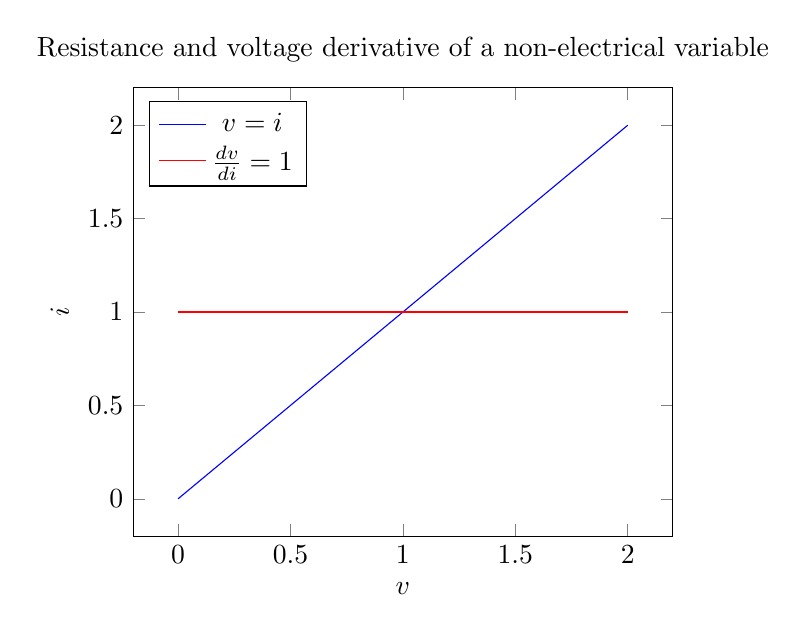
\begin{tikzpicture}
\begin{axis}[
    title={Resistance and voltage derivative of a non-electrical variable},
    xlabel={$v$},
    ylabel={$i$},
    domain=0:2,
    samples=100,
    legend pos=north west
]
\addplot [blue] {x}; % v = i (linear function)
\addlegendentry{$v = i$}

\addplot [red] {1}; % derivative of v = i (constant function)
\addlegendentry{$\frac{dv}{di} = 1$}
\end{axis}
\end{tikzpicture}
\end{displaymath}

\newpage

\section{Circuit Analysis}

\subsection{Kirchhoff's Laws}

\defn{Kirchhoff's Laws}{Kirchhoff's Laws are two fundamental laws that govern the behavior of electrical circuits.}

\emph{There is two things to consider: devices and topology restrictions.}

\begin{itemize}
  \item{Kirchhoff's Current Law (KCL)}
  \item{Kirchhoff's Voltage Law (KVL)}
  \item{Devices: resistors, capacitors, inductors, etc.}
\end{itemize}

\subsubsection{Kirchhoff's Current Law - KCL}

\defn{Kirchhoff's Current Law}{Kirchhoff's Current Law states that the sum of currents entering a node is equal to the sum of currents leaving a node.}

\begin{equation}
  \sum_{i=1}^{n} i_{\text{in}} = \sum_{i=1}^{n} i_{\text{out}}
\end{equation}


\begin{quote}

  The circuit diagrams above illustrate \emph{Kirchhoff's Current Law}(KCL), 
which states that the algebraic sum of currents entering a node (or a junction) equals zero. 
This principle is a consequence of the conservation of electric charge. 

In the first diagram, we see positive charges $(+)$ flowing into a node. Each arrow represents a current path, 
and the label $i_{\text{in}}^-$ indicates that these are incoming currents. In the second diagram, we see negative charges $(-)$ flowing out of a node, 
which represent electrons moving out of the node, creating a current. 

The arrows again indicate the direction of the current flow, and the label $i_{\text{out}}^-$ indicates that these are outgoing currents. According to KCL, 
the sum of the incoming currents should equal the sum of the outgoing currents at a node, which is visually represented in these diagrams.

\end{quote}

The graph below illustrates the concept of Kirchhoff's Current Law, showing the algebraic sum of currents entering a node equal to zero in the passive convention.

\begin{figure}[ht]
  \centering
  \begin{minipage}{.5\textwidth}
    \centering
    \begin{circuitikz}
      \draw (0,0) node[circ] {} -- (2,0) to[short, i=$i_{\text{in}}^-$] (1,0);
      \draw (0,0) -- (-2,0) to[short, i=$i_{\text{in}}^-$] (-1,0);
      \draw (0,0) -- (0,2) to[short, i=$i_{\text{in}}^-$] (0,1);
      \draw (0,0) -- (0,-2) to[short, i=$i_{\text{in}}^-$] (0,-1);
    \end{circuitikz}
    \caption{{Positive charges $(+)$ flowing into the node}}    
  \end{minipage}%
  \begin{minipage}{.5\textwidth}
    \centering
    \begin{circuitikz}
      \draw (0,0) node[circ] {} -- (1,0) to[short, i=$i_{\text{out}}^-$] (2,0);
      \draw (0,0) -- (-1,0) to[short, i=$i_{\text{out}}^-$] (-2,0);
      \draw (0,0) -- (0,1) to[short, i=$i_{\text{out}}^-$] (0,2);
      \draw (0,0) -- (0,-1) to[short, i=$i_{\text{out}}^-$] (0,-2);
    \end{circuitikz}
    \caption{{Negative charges $(-)$ flowing out of the node}}
  \end{minipage}
\end{figure}

\newpage

\subsubsection{Kirchhoff's Voltage Law - KVL}

\defn{Kirchhoff's Voltage Law}{Kirchhoff's Voltage Law states that the sum of voltages around a closed loop is equal to zero.}

\emph{At any closed loop, the sum of the voltage sources is equal to the sum of the voltage drops.}

\begin{equation}
  \sum_{i=1}^{n} v_{\text{in}} = \sum_{i=1}^{n} v_{\text{out}}
\end{equation}

\begin{quote}
The circuit diagram above represents a node with negative charges flowing out. This is a visualization of 
Kirchhoff's Current Law, which states that the algebraic sum of currents entering a node (or a junction) equals zero. 
In this case, the negative charges represent electrons moving out of the node, which creates a current. \\

The arrows indicate the direction of the current flow. Each arrow represents a current path, and the label \boldmath{$i_{\text{out}}^-$} 
indicates that these are outgoing currents. This diagram is a useful tool for understanding the behavior of electrical circuits, 
particularly the principle of conservation of electric charge, which is the basis of \emph{Kirchhoff's Current Law.}

\end{quote}

\emph{Sum of voltages around a closed loop is equal to zero independent of the direction of the loop.}
\begin{figure}[ht]
  \centering
  \begin{minipage}{.5\textwidth}
    \centering
    \begin{align}
      V_g &= V_1 + V_2 + V_3 \nonumber \\
      &= i_g \cdot R_1 + i_g \cdot R_2 + i_g \cdot R_3 \nonumber \\
      &= i_g \cdot (R_1 + R_2 + R_3) \nonumber \\
      &= i_g \cdot R_{\text{eq}}
  \end{align}
    \caption{{Circuit from $+$ to $-$}}
  \end{minipage}%
  \begin{minipage}{.5\textwidth}
    \centering
    \begin{align}
      V_g &= - V_1 - V_2 - V_3 \nonumber \\
      &\therefore \  R^{+}_{eq} \equiv R^{-}_{eq} \nonumber \\
  \end{align}
    \caption{{Circuit from $-$ to $+$}}
  \end{minipage}
\end{figure}

% example 1 here

\newpage
\subsubsection{{Example I. Kirchhoff's Laws in a Series Circuit with Resistors}}

Consider a simple series circuit with a DC power source and two resistors, as shown below, \textbf{assuming the passive convention}:

\begin{figure}[ht]
  \centering
  \begin{circuitikz}[american voltages]
    \draw (0,0) to[V, l=$V_g$, i=$i_g$] (0,2)
          to[R, l=$R_1$, v=$V_1$] (2,2)
          to[R, l=$R_2$, v=$V_2$] (4,2)
          -- (4,0) -- (0,0);
  \end{circuitikz}
  \caption{Series circuit with a DC power source and two resistors}
\end{figure}

According to Kirchhoff's Voltage Law (KVL), the sum of the voltages around any closed loop in the circuit is equal to zero. For this circuit, the equation is:

\begin{equation}
V_g = V_1 + V_2
\end{equation}

According to Ohm's law, the voltage across a resistor is equal to the current through the resistor times the resistance of the resistor. So we can write:

\begin{align}
V_1 &= i_g \cdot R_1 \\
V_2 &= i_g \cdot R_2
\end{align}

Substituting these equations into the KVL equation, we get:

\begin{equation}
V_g = i_g \cdot R_1 + i_g \cdot R_2 = i_g \cdot (R_1 + R_2)
\end{equation}

This equation tells us that the voltage of the power source is equal to the current through the circuit times the total resistance of the circuit.

According to Kirchhoff's Current Law (KCL), the sum of the currents entering a node (or a junction) equals the sum of the currents leaving the node. For this circuit, the equation is:

\begin{equation}
i_g = i_1 = i_2
\end{equation}

This equation tells us that the current through the power source is equal to the current through each resistor, which is a characteristic of series circuits.

It's important to note that the direction of the loop does not affect the application of KVL. Whether we move in the direction of the current (from $+$ to $-$) or against it (from $-$ to $+$), the sum of the voltages around the loop is still zero. This is true even in the presence of a power source or a load, where the power is negative or positive, respectively.


\newpage
\subsubsection{Example II. Proof that the direction of the loop does not affect the application of KVL}

Consider a simple series circuit with a DC power source and two resistors, as shown below, \textbf{assuming the passive convention}:

\begin{figure}[ht]
  \centering
  \begin{circuitikz}[american voltages]
    \draw (0,0) to[V, l=$V_g$, i=$i_g$] (0,2)
          to[R, l=$R_1$, v=$V_1$] (2,2)
          to[R, l=$R_2$, v=$V_2$] (4,2)
          -- (4,0) -- (0,0);
  \end{circuitikz}
  \caption{Series circuit with a DC power source and two resistors}
\end{figure}

Given the values:

\begin{itemize}
\item Voltage of the power source, $V_g = 12V$
\item Resistance of the first resistor, $R_1 = 2\Omega$
\item Resistance of the second resistor, $R_2 = 3\Omega$
\item Current through the circuit, $i_g = 2A$
\end{itemize}

We can calculate the voltage across each resistor using \textbf{Ohm's law}, $V = i \cdot R$:

\begin{align}
V_1 &= i_g \cdot R_1 = 2A \cdot 2\Omega = 4V \\
V_2 &= i_g \cdot R_2 = 2A \cdot 3\Omega = 6V
\end{align}

Now we can apply \textbf{KVL} in the direction of the current (from $+$ to $-$):

\begin{equation}
V_g - V_1 - V_2 = 0
\end{equation}

Substituting the given values:

\begin{equation}
12V - 4V - 6V = 2V \neq 0
\end{equation}

\textbf{This is not consistent with KVL}. The issue here is that the current $i_g$ is not correct. The current through the circuit should be equal to the voltage of the power source divided by the total resistance of the circuit, according to Ohm's law. So, the correct current is:

\begin{equation}
i_g = \frac{V_g}{R_1 + R_2} = \frac{12V}{2\Omega + 3\Omega} = 2.4A
\end{equation}

Substituting this current into the voltages across the resistors:

\begin{align}
V_1 &= i_g \cdot R_1 = 2.4A \cdot 2\Omega = 4.8V \\
V_2 &= i_g \cdot R_2 = 2.4A \cdot 3\Omega = 7.2V
\end{align}

Substituting these voltages into the KVL equation:

\begin{equation}
12V - 4.8V - 7.2V = 0V
\end{equation}

\textbf{Now, the sum of the voltages around the loop is equal to zero, which is consistent with KVL}. So, the direction of the loop does not affect the application of KVL, as long as we follow the passive sign convention and use the correct current.

